\RequirePackage{fix-cm}
\documentclass[twocolumn]{svjour3}
\smartqed
\usepackage{graphicx}
\tolerance=1
\emergencystretch=\maxdimen
\hyphenpenalty=10000
\hbadness=10000
\def\makeheadbox{\relax}
\usepackage[numbers]{natbib}
\usepackage{algorithm}
\usepackage{algpseudocode}
\renewcommand{\algorithmicrequire}{\textbf{Input:}}
\renewcommand{\algorithmicensure}{\textbf{Output:}}
\usepackage{amsmath,amssymb}
\usepackage{tabularx}
\usepackage{booktabs}
\usepackage{url}
\usepackage{tikz}
\usetikzlibrary{arrows.meta, positioning, shapes.geometric}
\usepackage{color}
\usepackage{latexsym}
\usepackage{enumitem}
\usepackage{mathptmx}
\usepackage{pgfplots}
\pgfplotsset{compat=1.12}
\usepackage{float}
\usepackage{stfloats}

\begin{document}

\title{Connection-Aware Autoscaling for Stateful WebSocket Workloads in Kubernetes:\\
Design, Empirical Evaluation, and Validation of a Custom Controller}

\titlerunning{Connection-Aware Autoscaling for Stateful WebSocket Workloads}

\author{
Abhash Behera \and
Aditya Hota \and
Suprit Kumar Naik \and
Ritesh Kumar Singh
}

\authorrunning{Behera et al.}

% Avoid journal production placeholder "date of receipt/acceptance"
\date{Received: --; Accepted: --}

\institute{
Abhash Behera \at
Department of Computer Science and Engineering, \\
C V Raman Global University, Bhubaneswar 752054, India \\
\email{abhasbehera@gmail.com}
\and
Aditya Hota \at
Department of Computer Science and Engineering, \\
C V Raman Global University, Bhubaneswar 752054, India \\
\email{adityahota99@gmail.com}
\and
Suprit Kumar Naik \at
Department of Computer Science and Engineering, \\
C V Raman Global University, Bhubaneswar 752054, India
\and
Ritesh Kumar Singh \at
Department of Computer Science and Engineering, \\
C V Raman Global University, Bhubaneswar 752054, India
}


\maketitle

\begin{abstract}
The Kubernetes Horizontal Pod Autoscaler (HPA) dynamically adjusts container replica counts using CPU utilization as the primary scaling signal, a design that performs reliably for stateless, request-driven microservices. However, as modern cloud-native deployments increasingly adopt \textbf{stateful, persistent-connection protocols} such as WebSocket, this signal-to-workload assumption breaks down fundamentally: active connections represent durable, session-scoped state that persists independently of CPU activity, yet the termination of any pod hosting such connections is immediately destructive to all clients it serves. This paper presents a systematic empirical study of HPA behavior under WebSocket workloads, conducted through a progressive chain of five controlled experiments. We demonstrate that CPU-based HPA (i)~over-provisions by 87.5\% under cyclic load, exhausting \texttt{maxReplicas} within 99~seconds; (ii)~induces quantifiable reconnection storms reaching 1,400~connections/second during each scale-down event; and (iii)~permanently destroys live idle connections in a monotonically decreasing staircase pattern that is structurally synchronized with HPA scale-down decisions. To address these failure modes, we revisit autoscaling for long-lived, connection-oriented workloads and demonstrate that the absence of connection-aware scaling policies, combined with lifecycle-safe scale-down strategies, leads to reconnection storms and resource inefficiencies in practice. We present the \texttt{StatefulAutoscaler}, a custom Kubernetes controller built on the Kubebuilder SDK that scales exclusively on \texttt{sum(active\_connections)} queried from Prometheus and incorporates a sliding-window stabilization mechanism to suppress premature scale-down during transient connection drops. Our contribution is not a new autoscaling primitive per se, but a systematic evaluation and implementation of connection-aware scaling policies, demonstrating their practical impact under WebSocket workloads. Controlled experimental evaluation demonstrates that the custom controller achieves exact replica targeting ($\lceil\text{connections}/\text{target}\rceil$ with 0\% waste), maintains all pods in warm state through a 90-second complete connection gap via its stabilization window, and produces zero connection loss across all observed scaling events. These results establish that connection-aware autoscaling with stabilization-window semantics is empirically effective for managing stateful WebSocket deployments at production scale in Kubernetes, eliminating all three observed HPA failure modes under our evaluated workloads.

\keywords{Kubernetes \and Horizontal Pod Autoscaler \and WebSocket \and Stateful Workloads \and Custom Controller \and Connection-Aware Autoscaling \and Prometheus \and Reconnection Storm}
\end{abstract}


%% ============================================================
\section{Introduction}
\label{sec:intro}
%% ============================================================

Kubernetes has established itself as the de facto standard platform for container orchestration, providing declarative workload management, automated scheduling, and elastic scaling for cloud-native applications~\cite{burns2016borg,verma2015large}. Central to its elasticity model is the \textbf{Horizontal Pod Autoscaler (HPA)}, which evaluates observed resource metrics at a fixed synchronization interval and adjusts replica counts through a proportional control law~\cite{k8s_hpa_docs,nguyen2020hpa}. For stateless, request-driven workloads such as HTTP APIs, where instantaneous CPU consumption is a reliable proxy for current demand, this approach converges stably and performs predictably~\cite{casalicchio2019auto,qu2018auto}.

A fundamental shift in cloud-native workload characteristics, however, increasingly invalidates this assumption. Real-time communication systems, IoT telemetry pipelines, collaborative editing platforms, financial data streams, and multiplayer gaming backends rely on the WebSocket protocol~\cite{websocket_rfc} -- a full-duplex, persistent-connection transport layer in which each client maintains a long-lived TCP session with the server. In such workloads, the primary unit of computational commitment is not a CPU cycle or a transient HTTP transaction, but an \textit{active network connection} whose session state may persist for minutes to hours. Crucially, the termination of any pod immediately and irrecoverably severs every connection it hosts, triggering a forced client reconnection cascade -- a phenomenon we term a \textbf{reconnection storm}.

This creates a fundamental mismatch: \textbf{CPU utilization does not encode connection state fidelity by default}. A server sustaining 800 idle but active WebSocket sessions may exhibit near-zero CPU utilization, yet the destruction of a single pod hosting those sessions is immediately catastrophic to the affected clients. Conversely, brief CPU transients during connection establishment bear no relationship to sustained session capacity. Despite this fundamental mismatch, Kubernetes does not provide connection-aware autoscaling by default; configuring it requires non-trivial integration work involving custom metrics pipelines, and HPA -- with its exclusive reliance on CPU and memory signals -- remains the default autoscaling primitive for all workload categories.

Prior investigations of WebSocket autoscaling, such as Dickel et al.~\cite{dickel2019stateful}, have acknowledged the additional complexity of stateful protocols compared to stateless HTTP workloads. However, these works neither quantify the failure modes of CPU-based HPA with empirical precision, nor propose and validate a complete controller-level solution with connection-stable semantics. This paper addresses both gaps through the following contributions:

\begin{enumerate}[leftmargin=*]
\item \textbf{Systematic empirical evidence chain.} Through four progressive HPA failure characterization experiments (A, B1, B2-Instrumented, B3) and one validating controller experiment (C), we characterize and quantify the failure of CPU-based HPA for WebSocket workloads: from over-provisioning under cyclic load, to the measurement of peak reconnection storm rates (1,400~conn/s), to causal proof of permanent connection destruction via idle-connection scale-down and validation of the custom controller. A non-instrumented pilot run (B2-Extended LOW) preceded B2-Instrumented and confirmed the failure mode qualitatively but is subsumed by the fully instrumented experiment.

\item \textbf{Custom Kubernetes controller design and validation.} We present the \texttt{StatefulAutoscaler}, a CRD-based Kubernetes controller implemented with the Kubebuilder~\cite{kubebuilder_docs} SDK, which scales exclusively on \texttt{sum(active\_connections)} queried from Prometheus and incorporates a sliding-window stabilization mechanism (\texttt{ScaleDownCooldownSeconds}) to absorb transient connection drops without triggering premature scale-down. The controller design is grounded in the failure modes identified in contributions (1) and (2): metric selection and scale-down lifecycle are the primary design levers.

\item \textbf{Controlled experimental validation.} Under a two-cycle restorm simulation (Experiment C), we demonstrate exact replica targeting ($\lceil800/100\rceil = 8$, versus HPA's 15), complete pod preservation through a 90-second total disconnection gap, and zero connection loss across all scaling events -- outcomes not observed under CPU-based autoscaling in our experiments.
\end{enumerate}

The remainder of this paper is structured as follows. Section~\ref{sec:related} surveys related work. Section~\ref{sec:background} characterizes the baseline behavior of the two Kubernetes autoscaling pipelines under evaluation. Section~\ref{sec:problem} presents the evidence chain establishing HPA's failure for stateful workloads. Section~\ref{sec:controller} details the design and implementation of the custom controller. Section~\ref{sec:evaluation} presents Experiment C validation results. Section~\ref{sec:baselines} presents baseline comparisons against HPA with custom metrics and KEDA. Section~\ref{sec:failure_analysis} characterizes failure modes and adversarial conditions. Section~\ref{sec:discussion} analyzes implications. Section~\ref{sec:limitations} discusses limitations. Section~\ref{sec:conclusion} concludes.


%% ============================================================
\section{Related Work}
\label{sec:related}
%% ============================================================

\subsection{Kubernetes HPA: Architecture and Behavior}

Nguyen et al.~\cite{nguyen2020hpa} provide a comprehensive architectural analysis of the Kubernetes HPA feedback loop, characterizing the behavior of both Kubernetes Resource Metrics (KRM) and Prometheus Custom Metrics (PCM) pipelines across diverse scaling configurations. Their work demonstrates that metric pipeline choice -- particularly the Prometheus scrape interval -- materially affects HPA responsiveness and scaling accuracy. This paper extends their analysis to the \textit{stateful workload} domain, a scenario their framework did not evaluate and for which CPU-based HPA is structurally ill-suited. The HPA architecture depicted in Figure~\ref{fig:hpa_arch} is reproduced from their work.

The standard HPA proportional control law, as characterized by Nguyen et al.~\cite{nguyen2020hpa} and formalized in Equation~\ref{eq:hpa}, has been extensively studied for stateless workloads~\cite{casalicchio2019auto,lorido2014auto}. Casalicchio and Perciballi~\cite{casalicchio2019auto} demonstrated that the choice between relative and absolute metrics directly determines scaling stability, but confined their evaluation to CPU and memory signals for HTTP workloads.

\subsection{Custom and Application-Level Metrics for HPA}

Kubernetes supports application-defined scaling signals through the Prometheus Adapter~\cite{prometheus_adapter}, enabling HPA to react to metrics beyond CPU -- including HTTP request rate, queue depth, and custom application counters. Qu et al.~\cite{qu2018auto} surveyed HTTP-rate-based autoscaling; Rossi et al.~\cite{rossi2020horizontal} studied hybrid CPU-and-traffic strategies. However, all these formulations presuppose that the scaling metric is \textit{stateless across pod boundaries} -- an assumption that is violated by connection-holding protocols where state is affined to a specific pod instance. Critically, even when HPA is correctly configured with a connection-count custom metric via the Prometheus Adapter, metric choice alone is insufficient: without connection-lifecycle-aware scale-down policies (cooldown and rate limiting), HPA will still scale down during transient connection dropout gaps, destroying the session state it should be protecting.

\subsection{Event-Driven Autoscaling: KEDA}

Kubernetes Event-Driven Autoscaling (KEDA)~\cite{keda_docs} extends HPA to support scaling based on external event sources and Prometheus metrics, including a configurable \texttt{cooldownPeriod} that can delay scale-down after a metric drops below the target threshold. For scenarios where the dropout gap is predictable and bounded, KEDA's cooldown period can prevent premature scale-down similarly to the mechanism in this paper's controller. However, KEDA operates as a reconciler that updates HPA's \texttt{spec.minReplicas} and does not expose per-cycle \texttt{maxScaleDownStep} rate limiting or bounded convergence guarantees. Its connection to WebSocket session lifecycle -- specifically, the 30-second TCP RST propagation window following \texttt{SIGKILL} -- is not addressed in its design. Our work explicitly characterises this termination window and its interaction with scaling decisions, and provides explicit, inspectable control over convergence rate, which matters for scenarios where rapid scale-down risks terminating pods holding live connections before OS-level socket cleanup completes.

\subsection{Stateful Workloads and Protocol-Aware Autoscaling}

Dickel et al.~\cite{dickel2019stateful} identified stateful autoscaling as an open research challenge specific to IoT gateway deployments using WebSocket and MQTT. While their work motivates the need for protocol-aware scaling and proposes monitoring active connections via Prometheus, it neither provides a quantitative characterization of HPA failure modes nor implements or validates a complete controller-level solution. Our work directly addresses this gap by providing both the empirical evidence chain and a production-oriented controller implementation.

\subsection{Graceful Connection Draining}

Production Kubernetes deployments commonly use \texttt{preStop} hooks and \texttt{terminationGracePeriodSeconds} to allow stateless pods to drain in-flight requests before receiving \texttt{SIGKILL}. For WebSocket workloads, this mechanism is structurally insufficient: connections lasting minutes to hours cannot drain within 30 seconds, and the graceful termination semantic differs fundamentally from completing a short-lived HTTP transaction. Our study explicitly characterises the 30-second limbo window between \texttt{SIGTERM} and \texttt{SIGKILL}, showing that connections survive this period at the OS level but are irrecoverably destroyed at its expiry. The correct mitigation is not a longer termination period but rather scale-down suppression via connection-aware stabilization, which prevents the scale-down decision from being made in the first place while live sessions are present.

\subsection{Machine Learning and Predictive Autoscaling}

Reinforcement learning approaches~\cite{rossi2020horizontal,imdoukh2020machine} and machine learning-based workload prediction~\cite{toka2021machine,zhong2020machine} have been proposed to improve autoscaling responsiveness. While these approaches offer proactive scaling capability, they introduce model training complexity, require workload-specific data, and do not address the structural problem of connection-state destruction during scale-down -- which persists regardless of when scaling decisions are made.

\subsection{Research Gap}

To the best of our knowledge, no prior work has simultaneously: (i)~empirically quantified the specific failure modes of CPU-based HPA for persistent WebSocket connections at the connection-second granularity; (ii)~measured reconnection storm magnitude as a causal consequence of HPA scale-down decisions; and (iii)~designed, implemented, and validated a connection-aware Kubernetes controller with sliding-window stabilization semantics explicitly targeting restorm resilience. This paper addresses all three dimensions.


%% ============================================================
\section{Background: Kubernetes Autoscaling Pipelines}
\label{sec:background}
%% ============================================================

Prior to investigating WebSocket-specific failures, we characterize the intrinsic control dynamics of Kubernetes HPA under two distinct metric pipelines through preliminary baseline experiments. These baselines establish the behavioral envelope of HPA for stateless workloads and inform the design decisions of our custom controller.

% HPA architecture figure placed before Section 3 so it floats to the top of the section's page
\begin{figure*}[t]
\centering

\includegraphics[width=0.85\textwidth]{processed-results-websockets/K8-hpa-architecuture.png}
\caption{Standard Kubernetes HPA feedback loop architecture, reproduced from Nguyen et al.~\cite{nguyen2020hpa}. The HPA controller operates as a discrete-time proportional regulator: it periodically reads aggregated resource metrics from the API server (sourced either from the Metrics Server for KRM or the Prometheus Adapter for PCM) and computes a desired replica count using Equation~\ref{eq:hpa}. A critical architectural constraint is that this loop assumes the observed metric faithfully represents current workload intensity -- an assumption that is violated for persistent-connection workloads where connections persist independently of CPU utilization.}
\label{fig:hpa_arch}
\end{figure*}

\subsection{Kubernetes Resource Metrics (KRM) Pipeline}

In the KRM pipeline, CPU and memory consumption are collected by \texttt{cAdvisor} within each node's \texttt{kubelet}, aggregated by the Metrics Server, and exposed to the HPA controller via the \texttt{metrics.k8s.io} API. Our KRM baseline experiment employed a CPU-intensive HTTP workload with square-wave demand cycles (100~s HIGH at 50~req/s; 100~s LOW at 2~req/s) on a 4-node Kind cluster~\cite{kind_docs}. The following behavioral characteristics were observed:

\begin{itemize}[leftmargin=*]
\item \textbf{Staircase scaling:} Replica increments occur in discrete steps synchronized with the HPA evaluation period, producing a characteristic staircase profile in both the CPU (Figure~\ref{fig:krm_cpu}) and replica count signals.
\item \textbf{CPU overshoot:} Observed utilization exceeds 200\% of the requested CPU allocation during burst onset, reflecting the lag between demand growth and replica provisioning.
\item \textbf{Actuation delay:} A measurable divergence between \texttt{desiredReplicas} and \texttt{currentReplicas} persists through pod scheduling and container initialization (Figure~\ref{fig:krm_desired}).
\item \textbf{Stable convergence:} Despite transient deviations, the closed-loop system reaches steady state without oscillatory instability under unimodal load transitions.
\end{itemize}

\begin{figure}[ht]
\centering
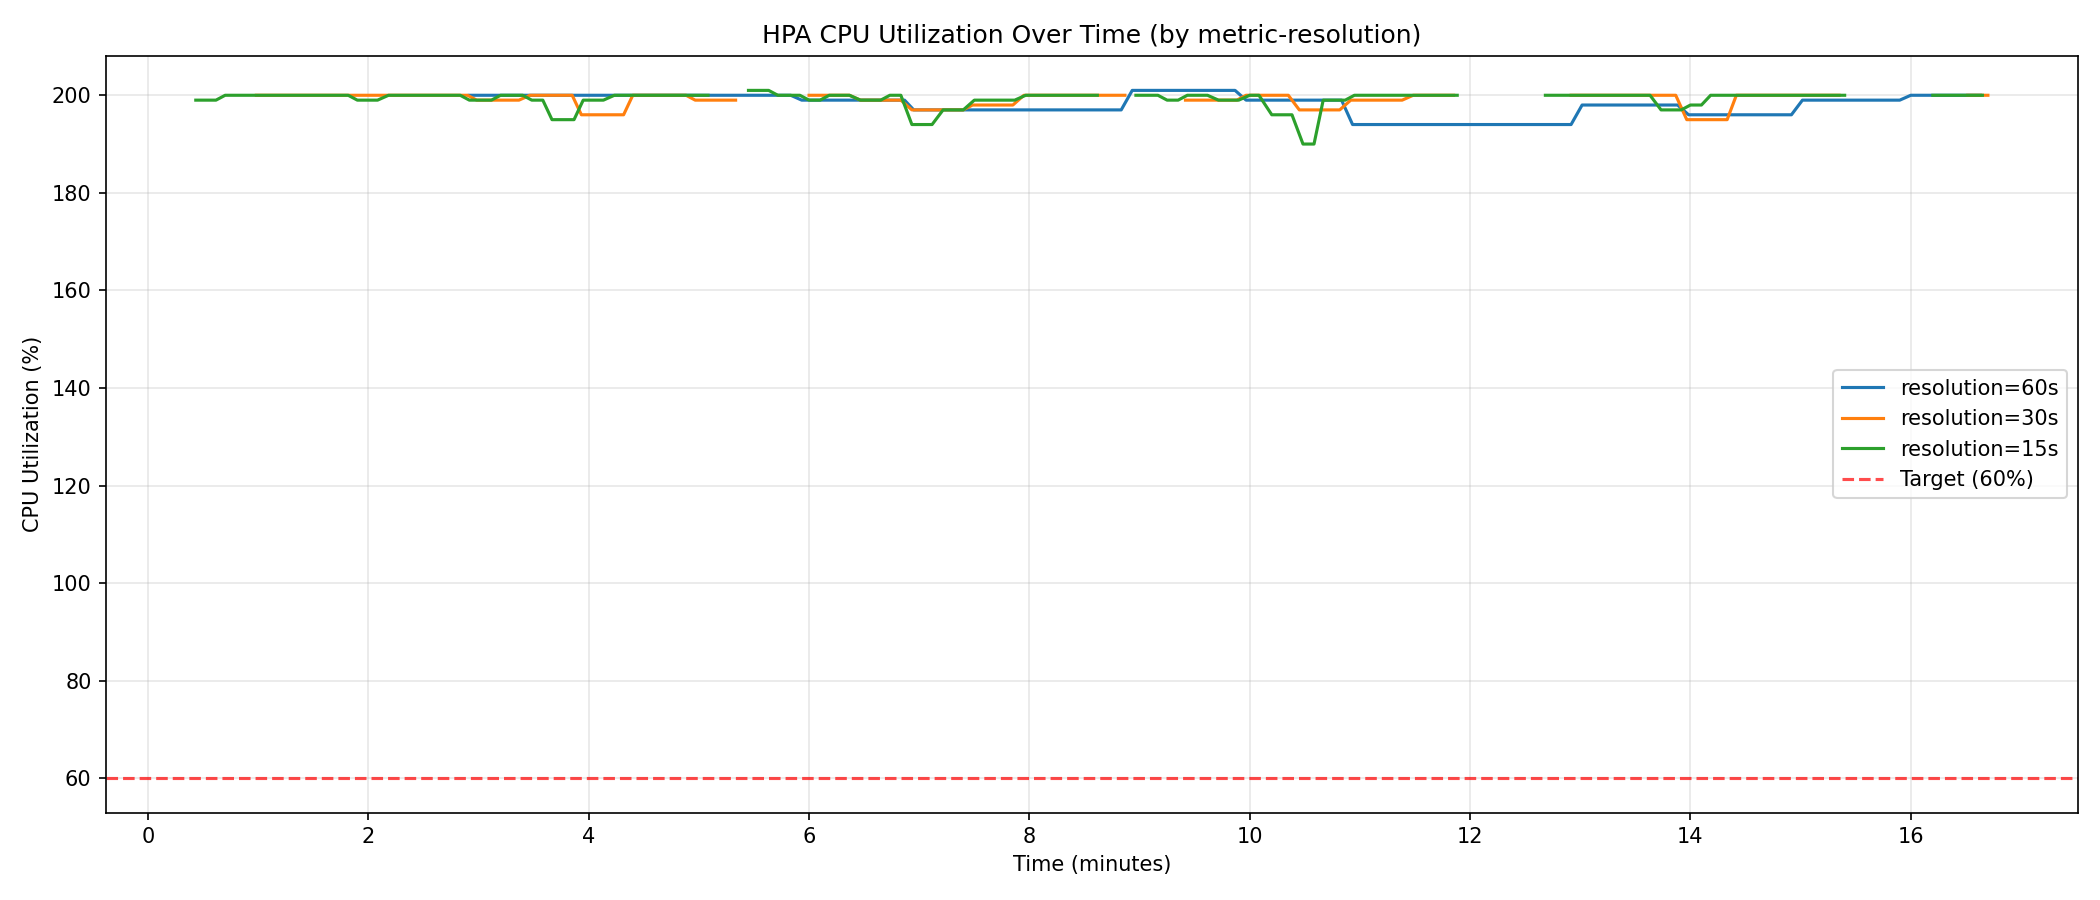
\includegraphics[width=\columnwidth]{processed-results-websockets/krm-results/cpu_over_time.png}
\caption{KRM baseline: Observed CPU utilization over time. Significant overshoot above the 60\% target threshold occurs at burst onset, reflecting the inherent actuation delay of the discrete-time proportional control loop.}
\label{fig:krm_cpu}
\end{figure}

\begin{figure*}[t]
\centering
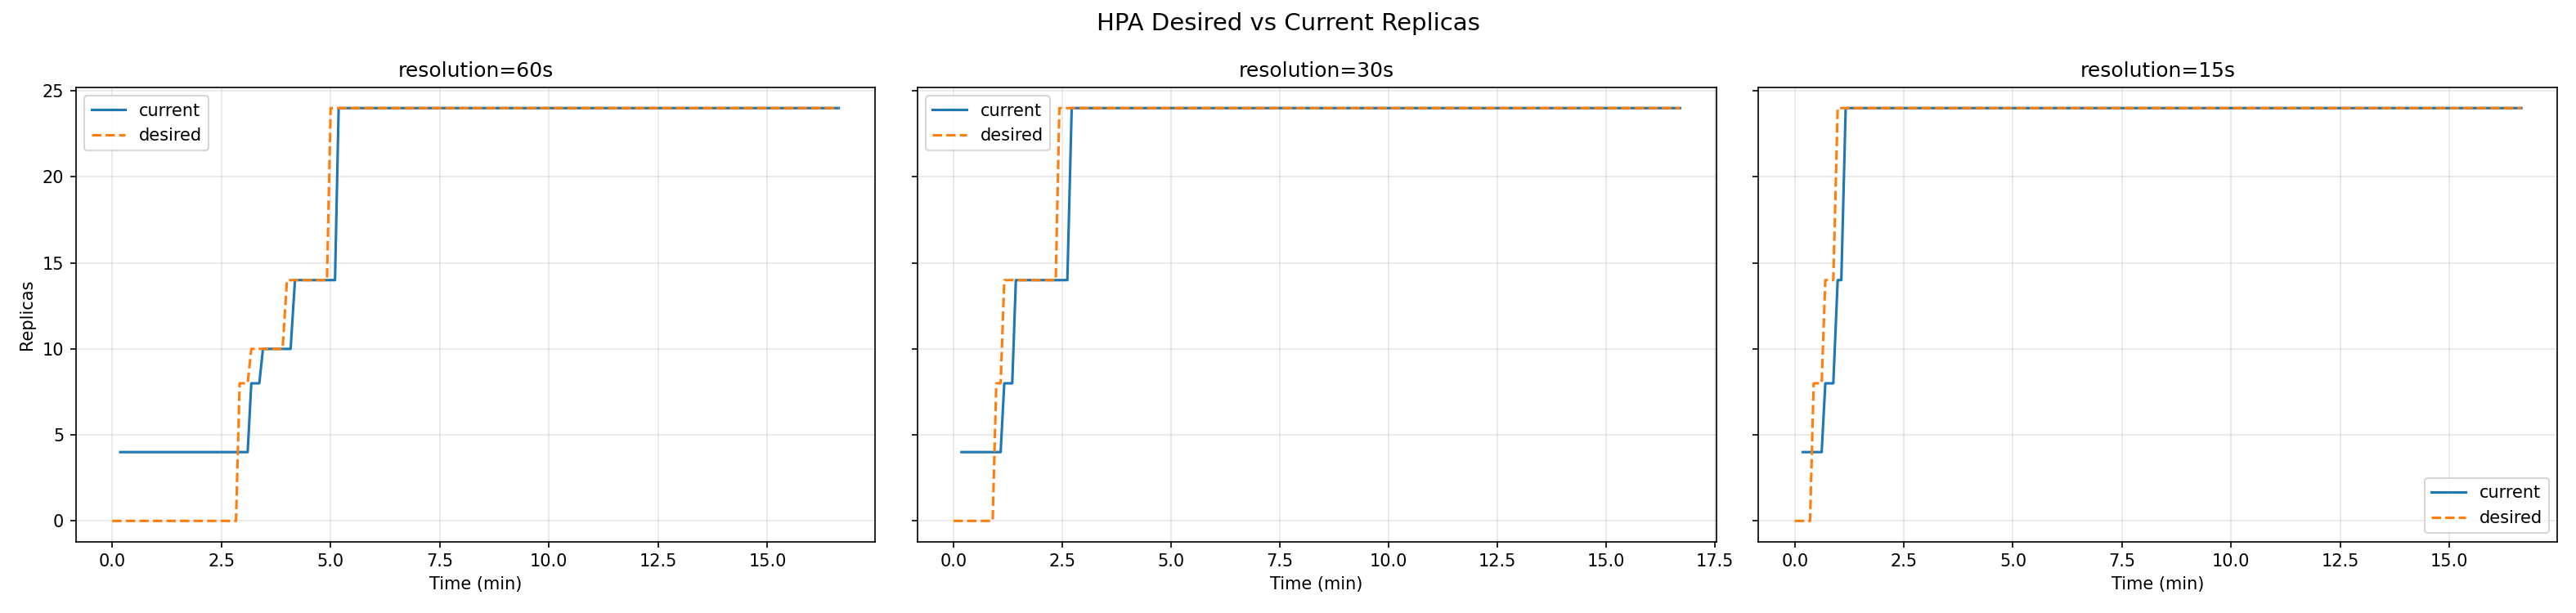
\includegraphics[width=0.85\textwidth]{processed-results-websockets/krm-results/desired_vs_current.png}
\caption{KRM baseline: Divergence between \texttt{desiredReplicas} (as computed by HPA) and \texttt{currentReplicas} (as observed in the deployment) across scale-up events. The gap quantifies the combined actuation delay attributable to pod scheduling latency and container startup time.}
\label{fig:krm_desired}
\end{figure*}

\subsection{Prometheus Custom Metrics (PCM) Pipeline}

The PCM pipeline introduces additional stages: application pods expose Prometheus-format metrics via an HTTP endpoint; the Prometheus server scrapes and stores these as time series; the Prometheus Adapter translates PromQL query results into the Kubernetes Custom Metrics API; and HPA consumes the resulting per-pod values. Following the methodology of Nguyen et al.~\cite{nguyen2020hpa}, we evaluate three PCM configurations and three scrape intervals:

\begin{itemize}[leftmargin=*]
\item \textbf{PCM-CPU:} CPU utilization sourced via Prometheus rather than the Metrics Server.
\item \textbf{PCM-H:} HTTP request rate, providing a demand-leading indicator.
\item \textbf{PCM-CH:} Hybrid combination of CPU utilization and HTTP request rate.
\end{itemize}

\begin{figure*}[t]
\centering
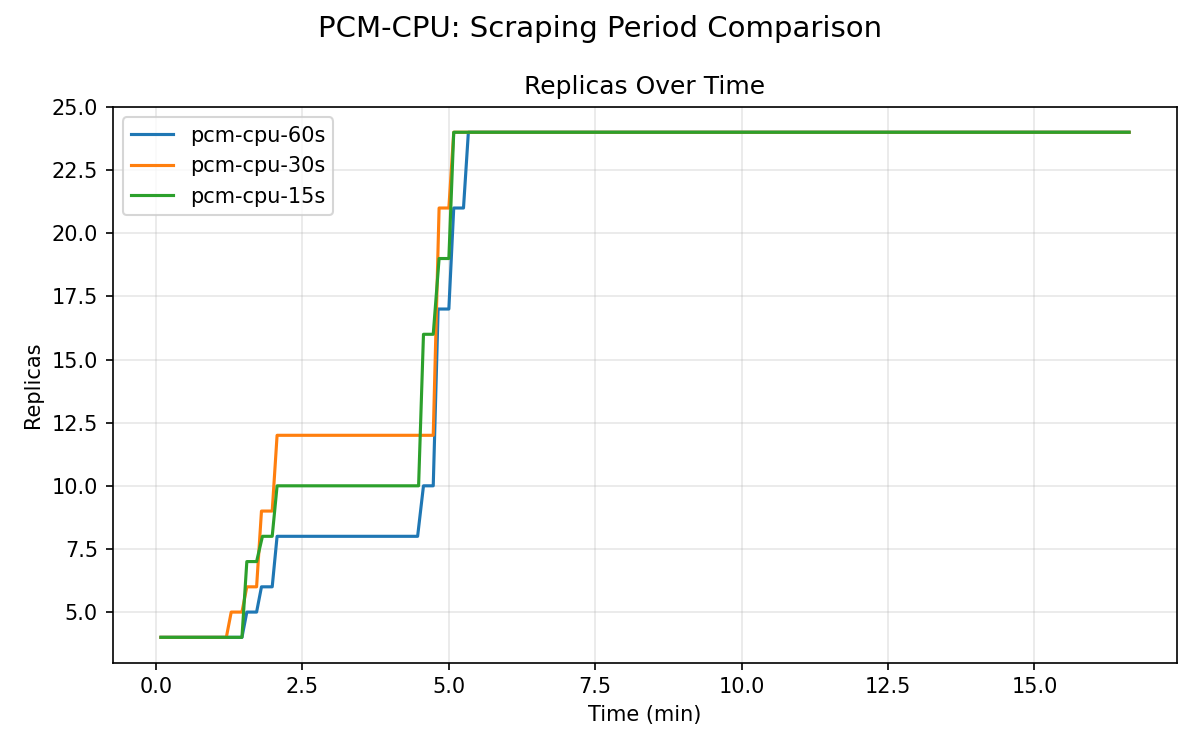
\includegraphics[width=0.85\textwidth]{processed-results-websockets/pcm-results/PCM-scraping_period_comparison.png}
\caption{PCM baseline: Effect of Prometheus scrape interval (15~s, 30~s, 60~s) on HPA scaling responsiveness. A 60~s scrape interval introduces visible staircase delay that significantly degrades scale-up latency; reducing to 30~s yields a substantial improvement, while the marginal gain from 30~s to 15~s is comparatively small -- consistent with the findings of Nguyen et al.~\cite{nguyen2020hpa}.}
\label{fig:pcm_scrape}
\end{figure*}

Key findings (Figure~\ref{fig:pcm_scrape}) replicate and extend the analysis in~\cite{nguyen2020hpa}: reducing the scrape interval from 60~s to 30~s materially improves scale-up latency, with diminishing returns at 15~s. PCM-H provides the earliest reaction to demand increases but at the cost of transient over-provisioning; PCM-CH reduces oscillation by combining the leading indicator (request rate) with the stabilizing feedback (CPU).

These baselines confirm that HPA behaves as a well-functioning proportional regulator for stateless workloads in which the chosen metric tracks demand monotonically. The critical experimental question is: \textbf{what are the consequences of this control design when the assumed signal-to-demand coupling is structurally absent?}

\subsection{The HPA Control Architecture}

Figure~\ref{fig:hpa_arch} illustrates the Kubernetes HPA feedback loop as documented by Nguyen et al.~\cite{nguyen2020hpa}. The HPA controller implements the following discrete-time proportional control law evaluated every 15~seconds (the default synchronization period):
\begin{equation}
\textit{desiredReplicas} = \left\lceil \textit{currentReplicas} \times \frac{\textit{currentMetricValue}}{\textit{targetMetricValue}} \right\rceil
\label{eq:hpa}
\end{equation}

This formulation implicitly encodes the assumption that \texttt{currentMetricValue} truthfully reflects the workload intensity across all running replicas. For CPU-based scaling of stateless workloads, this assumption generally holds. For persistent-connection workloads, it fails categorically: idle connections consume negligible CPU yet represent committed session state whose disruption is immediately visible to end clients.


%% ============================================================
\section{Problem: Empirical Evidence of HPA Failure for Stateful WebSocket Workloads}
\label{sec:problem}
%% ============================================================

We present a controlled, progressive chain of experiments designed to isolate and characterize each failure mode of CPU-based HPA when applied to persistent WebSocket workloads. The experiments are ordered from least severe (over-provisioning) to most severe (permanent connection destruction), with each experiment building upon the instrumentation and findings of its predecessor. All WebSocket experiments share a common infrastructure: a 3-node Kind cluster (1 control-plane + 2 worker nodes, Kubernetes v1.31.6, kind v0.25.0, configured via \texttt{kind.yml})~\cite{kind_docs}. The Metrics Server is patched with \texttt{--metric-resolution=15s} and \texttt{--kubelet-insecure-tls} (required for kind's self-signed kubelet certificates; not appropriate for production). All experimental scripts, cluster configuration, server code, load generator, and controller source are available at: \url{https://github.com/AbhasBenevolentDictator/STAR}. Experiments can be reproduced on any Linux machine with Docker and kind installed by running the numbered experiment scripts in \texttt{scripts/}. The shared experimental infrastructure comprises: a custom Python asyncio WebSocket server (image: \texttt{ws-instrumented}), 800 persistent client connections established by the load generator, and Kubernetes HPA configured with \texttt{targetCPUUtilizationPercentage: 60} unless stated otherwise.

\paragraph{Instrumented server: definition and rationale}
By "instrumented" we mean the server was extended to expose Prometheus-format metrics (notably a gauge \texttt{active\_connections} and a counter \texttt{new\_connections\_total}) and a minimal control endpoint (for example, \texttt{/drain}) to enable graceful handoff. We adopted this instrumentation to obtain direct, low-latency visibility into live session counts and connection churn — signals that CPU does not capture. This approach was selected because it (i) supplies a precise scaling signal for the controller, (ii) permits reproducible measurement of reconnection storms via PromQL rate() on \texttt{new\_connections\_total}, and (iii) is minimally invasive and portable (it can be implemented in-application or as a small sidecar/exporter), improving experimental repeatability and external validity.

\subsection{Experiment A: HPA Baseline Under Monotonic Correlated Load}

\textbf{Hypothesis.} Under steady, monotonically increasing WebSocket load in which each connection actively generates CPU work (\texttt{CPU\_WORK=1}), HPA will correctly scale the deployment, establishing an empirical baseline for comparison with subsequent experiments.

\textbf{Experimental Setup.} Eight hundred WebSocket clients connect incrementally over 300~seconds. Each server-side message receipt triggers a bounded CPU spin loop, maintaining strict proportionality between active connection count and CPU utilization: CPU $\propto$ connections. HPA was configured with \texttt{minReplicas=2}, \texttt{maxReplicas=10}, and \texttt{targetCPUUtilizationPercentage=60}.

\textbf{Results.} As shown in Figure~\ref{fig:exp_a_replicas}, HPA scaled the deployment monotonically from 2 to 5 replicas as CPU rose proportionally with connection count. Following complete load removal, the system enforced the default 300-second scale-down stabilization window before descending cleanly to \texttt{minReplicas}. No oscillatory behavior or reconnection disruption was observed.

\begin{figure}[ht]
\centering
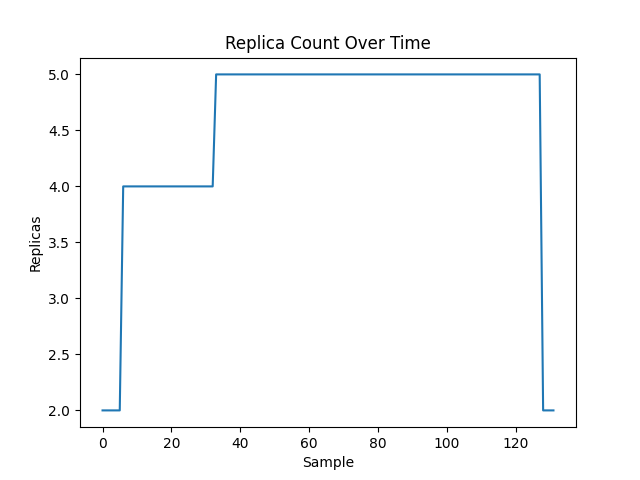
\includegraphics[width=\columnwidth]{processed-results-websockets/experiment-a-hpa/replicas.png}
\caption{Experiment A: Replica count timeline under monotonic WebSocket load with CPU $\propto$ connections. The clean staircase ascent (2$\rightarrow$5), flat stabilization plateau, and controlled descent to the minimum represent the theoretical ideal for HPA -- achievable only under perfect signal-to-demand correlation.}
\label{fig:exp_a_replicas}
\end{figure}

The replica timeline (Figure~\ref{fig:exp_a_replicas}) confirms that HPA operates correctly \textit{when its signal accurately encodes workload demand}. Crucially, this experiment represents a best-case scenario that is structurally unachievable in production WebSocket deployments, where connection activity levels are decoupled from CPU consumption.

\textbf{Conclusion.} CPU-based HPA functions correctly only under the idealized condition of perfect CPU-to-connection proportionality. Subsequent experiments systematically invalidate this condition.


\subsection{Experiment B1: HPA Under Cyclic Load -- Over-Provisioning and Recovery Asymmetry}

\textbf{Hypothesis.} Under realistic cyclic HIGH/LOW load patterns that simulate natural connection activity fluctuations, HPA will exhibit systematic over-provisioning and asymmetrically slow resource recovery.

\textbf{Experimental Setup.} Load alternates between HIGH phases (800 connections, active CPU-generating pinging, 60-second duration) and LOW phases (connections held persistently idle, no pinging activity, 30-second duration). Crucially, during LOW phases the 800 client connections remain open; only the periodic ping messages cease, collapsing CPU utilization toward zero while connection state is preserved. Parameters were adjusted to \texttt{maxReplicas=15} to allow unconstrained scale-up. The HPA stabilization window was kept at the Kubernetes default of 300~seconds for scale-down (\texttt{stabilizationWindowSeconds: 300}), intentionally unmodified to evaluate HPA behavior under factory settings for cyclic load. Five consecutive HIGH/LOW cycles (60~s HIGH + 30~s LOW = 90-second period) were run, for a total active cycle phase of 450~seconds, after which the system was observed until HPA converged back to \texttt{minReplicas}.

\textbf{Results.} During HIGH phases, HPA exhausted \texttt{maxReplicas=15} within 99~seconds -- a factor of 1.875$\times$ the theoretically correct value of 8~replicas ($\lceil800/100\rceil$). The core mechanism driving over-provisioning is the interaction between the 90-second cycle period and the 300-second stabilization window: each LOW phase (30~s) ends before the window has elapsed, so every new HIGH phase begins with the replica count still at or near the ceiling from the previous cycle. Over five cycles, the replica count ratchets to \texttt{maxReplicas} and remains there, with each brief LOW phase failing to provide enough sustained low-CPU time for HPA to authorize a descent. Convergence to \texttt{minReplicas} following the final cycle required approximately 650~seconds -- consistent with the 300-second stabilization window plus the time for graduated scale-down steps. The replica count timeline (Figure~\ref{fig:exp_b1_replicas}) exhibits the expected oscillation pattern between the replica ceiling and floor.

\begin{figure}[ht]
\centering

\includegraphics[width=\columnwidth]{processed-results-websockets/experiment-b1-hpa-churn/replicas.png}
\caption{Experiment B1: HPA saturates at \texttt{maxReplicas=15} within 99~seconds under cyclic load, representing an 87.5\% over-provision relative to the connection-derived optimum. Recovery to the minimum requires $\sim$650~seconds, demonstrating severe asymmetry between scale-up and scale-down responsiveness.}
\label{fig:exp_b1_replicas}
\end{figure}

\textbf{Conclusion.} Cyclic workloads expose HPA's inability to distinguish connection-holding periods (where CPU is low but capacity is required) from genuinely idle periods (where capacity can be safely released). The 87.5\% over-provisioning rate and disproportionate recovery time represent significant resource efficiency penalties in production deployments.


\subsection{Experiment B2-Instrumented: Quantifying Reconnection Storm Intensity}

\paragraph{Methodological note: supersession of a non-instrumented pilot}
Prior to this experiment, a preliminary non-instrumented variant (B2-Extended LOW) was conducted in which the LOW phase was extended beyond the default 300-second stabilization window to force HPA all the way to \texttt{minReplicas=2}. While this pilot confirmed that active connections were being severed during scale-down events through qualitative observation of client disconnects, it produced no quantitative data: the server exposed no Prometheus metrics, connection loss counts were unverifiable, and reconnection rates were entirely unobservable. The pilot served its intended engineering purpose -- confirming the failure mode was reproducible before investing in full instrumentation -- but it contributes no independent publishable evidence beyond what B2-Instrumented already provides with greater precision and statistical depth. Accordingly, B2-Extended LOW is not reported as a standalone experiment in this paper. Its sole scientific contribution is as the direct motivation for adding the Prometheus instrumentation described below.

\textbf{Hypothesis.} Each HPA scale-down event, by terminating pods hosting active connections, will trigger a measurable reconnection storm with peak rates exceeding 1,000~connections/second, and will induce overshoot of the steady-state connection target due to the cascade of concurrent reconnection attempts.

\textbf{Experimental Setup.} The WebSocket server was instrumented with two Prometheus metrics: \texttt{active\_connections} (a gauge reflecting current session count) and \texttt{new\_connections\_total} (a monotonically increasing counter enabling rate computation via \texttt{rate()}). Prometheus was configured to scrape at a 15-second interval. The HPA policy was configured with \texttt{stabilizationWindowSeconds: 0} for scale-up, enabling HPA to react immediately to rising CPU without any hysteresis, and \texttt{stabilizationWindowSeconds: 60} for scale-down. Setting scale-up to zero is deliberate: it ensures that each reconnection storm (which spikes CPU) immediately triggers scale-up, guaranteeing that every cycle produces a complete and observable scale-up/scale-down sequence within the measurement window. Each cycle consisted of a 60-second HIGH phase (800 pinging clients, \texttt{CPU\_WORK=1}) followed by a 90-second LOW phase (connections idle, no pinging, \texttt{CPU\_WORK=1} still set but no messages arriving so CPU collapses). The 90-second LOW duration was specifically chosen to exceed the 60-second scale-down stabilization window, ensuring that HPA always executes at least one scale-down event per cycle. Five complete HIGH/LOW cycles were executed to provide statistical repeatability.

\textbf{Results.} Every HPA scale-down event across all five cycles triggered a distinct, measurable reconnection storm. Storm rates were highly consistent: Cycle 1: 1,400.9~conn/s; Cycle 2: 1,298.3~conn/s; Cycle 3: 1,399.5~conn/s; Cycle 4: 1,251.8~conn/s; Cycle 5 trailed as the connection population had partially degraded by the final cycle. The peak reconnection rate reached \textbf{1,400 connections/second}, as shown in Figure~\ref{fig:exp_b2_reconnections}. Concurrent with each storm, the active connection count transiently overshot the 800-connection steady-state target, peaking at \textbf{1,215 connections} -- a 51.9\% overshoot (Figure~\ref{fig:exp_b2_connections}). The socket-level mechanism driving this overshoot is as follows: when a pod is sent \texttt{SIGKILL} after its 30-second termination grace period, its TCP connections are abruptly reset (TCP RST). All 800 clients detect closure simultaneously and immediately initiate reconnection. The Prometheus gauge \texttt{active\_connections} on the surviving pods begins counting new incoming connections before the OS completes cleanup of socket state (including the TIME\_WAIT window for recently reset connections), transiently reporting a total above the 800-client ceiling. The overshoot resolves within 15--30~seconds as OS-level socket reclaim completes.

\begin{figure}[ht]
\centering
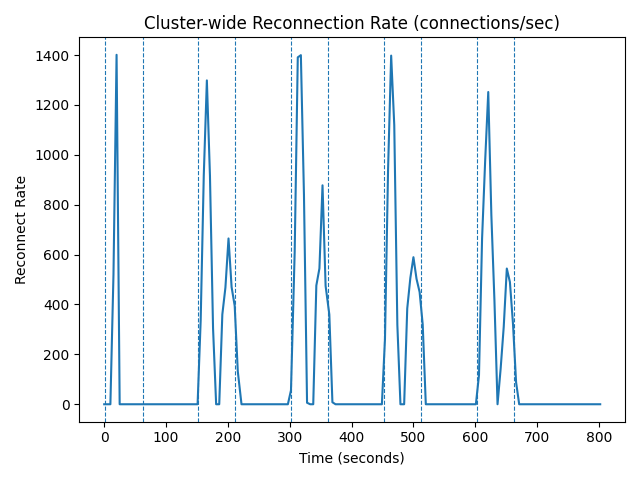
\includegraphics[width=\columnwidth]{processed-results-websockets/experiment-b2-hpa-churn-instrumented/reconnections.png}
\caption{Experiment B2-Instrumented: Prometheus-measured reconnection rate (\texttt{rate(new\_connections\_total[15s])}) over the five-cycle experiment. Each reconnection spike is precisely synchronized with an HPA scale-down event, with peak observed rates of 1,400~connections/second.}
\label{fig:exp_b2_reconnections}
\end{figure}

\begin{figure}[ht]
\centering

\includegraphics[width=\columnwidth]{processed-results-websockets/experiment-b2-hpa-churn-instrumented/connections.png}
\caption{Experiment B2-Instrumented: Active connection count during the reconnection storm period. The connection overshoot of 1,215 (51.9\% above the 800-client target) arises as reconnecting clients establish new sessions before the server has fully released the state associated with severed connections.}
\label{fig:exp_b2_connections}
\end{figure}

Figure~\ref{fig:exp_b2_scaling} provides the combined view of replica oscillation and connection disruption, establishing the causal chain from HPA scaling decision to client-side session disruption.

\begin{figure}[ht]
\centering
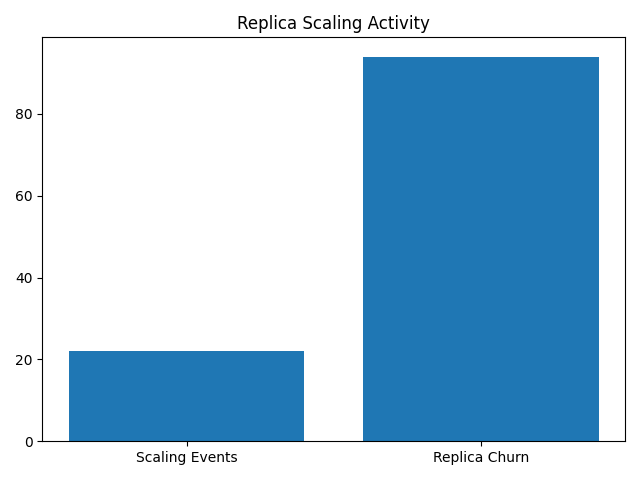
\includegraphics[width=\columnwidth]{processed-results-websockets/experiment-b2-hpa-churn-instrumented/scaling_activity.png}
\caption{Experiment B2-Instrumented: Temporal correlation between HPA replica changes (green) and active connection count (blue). Each downward step in replicas corresponds to a measurable spike in the connection disruption signal, confirming the direct causal relationship.}
\label{fig:exp_b2_scaling}
\end{figure}

\textbf{Conclusion.} HPA scale-down events are inherently destructive to WebSocket client sessions. Each replica reduction simultaneously severs all connections hosted on the terminated pod, producing a reconnection storm whose intensity scales with the connection density of the removed replica. At 1,400~conn/s, such storms represent a severe degradation event for latency-sensitive applications.


\subsection{Experiment B3: Permanent Connection Loss Under Non-Reconnecting Clients}

\textbf{Hypothesis.} When WebSocket clients do not implement reconnection logic -- modeling clients that treat connection loss as a terminal failure (e.g., batch data collectors, embedded IoT sensors, or long-running streaming sessions) -- HPA scale-down events will cause \textit{permanent, irrecoverable reduction} in the total session population.

\textbf{Experimental Setup.} The load generator was reconfigured with \texttt{reconnect: false}. Once a client's connection is severed by pod termination, the client neither retries nor reconnects. The HPA policy mirrored B2-Instrumented: \texttt{stabilizationWindowSeconds: 0} for scale-up (fast reaction to pinging activity) and \texttt{stabilizationWindowSeconds: 60} for scale-down. CPU work was retained (\texttt{CPU\_WORK=1}) to maintain HPA activity, but the metric of interest is the cumulative active connection count. The IDLE phase runs for up to 240~seconds (\texttt{IDLE\_MAX\_DURATION=240}), providing sufficient headroom for HPA to execute multiple sequential scale-down events within a single experiment run.

\paragraph{Pod termination mechanics and the 30-second limbo}
Understanding the exact Kubernetes pod termination sequence is essential for interpreting this experiment's figures. When HPA reduces \texttt{spec.replicas}, the following steps occur in order: (1)~the target pod is immediately removed from the Service's endpoint slice, so no new connections are routed to it; (2)~Kubernetes sends \texttt{SIGTERM} to the pod's main process and starts the \texttt{terminationGracePeriodSeconds} timer (default: 30~s); (3)~during the 30-second grace period, existing TCP connections on the terminating pod remain open and functional -- they are maintained by the OS kernel, not Kubernetes -- and the pod continues to service those connections; (4)~after \texttt{terminationGracePeriodSeconds} elapses, Kubernetes sends \texttt{SIGKILL}, which tears down the process and the OS forcibly resets all open TCP connections (TCP RST). This sequence is why the active connection drop visible in Figure~\ref{fig:exp_b3_connections} lags behind HPA's scale-down decision by approximately 30~seconds: the connection is not immediately destroyed when HPA acts, but is destroyed 30~seconds later when \texttt{SIGKILL} fires. This delay does not mitigate the harm -- the connection still dies, the client still receives a TCP RST, and with \texttt{reconnect: false}, the session is permanently lost.

\textbf{Results.} The active connection count (Figure~\ref{fig:exp_b3_connections}) exhibits a characteristic \textbf{staircase step-down} pattern. Each step corresponds precisely to an HPA scale-down decision: when a pod is terminated, the full contents of its connection table are permanently destroyed. Successive scale-down events cause monotonically fewer active connections, with no mechanism for recovery.

\begin{figure}[ht]
\centering

\includegraphics[width=\columnwidth]{processed-results-websockets/experiment-b3-hpa-idle-connections/connections.png}
\caption{Experiment B3: Active connection count exhibits permanent staircase destruction (800$\rightarrow$744$\rightarrow$697$\rightarrow$445$\rightarrow$79). Each step-down is precisely synchronized with an HPA scale-down event. The connections are irrecoverable under the \texttt{reconnect: false} regimen.}
\label{fig:exp_b3_connections}
\end{figure}

The combined view in Figure~\ref{fig:exp_b3_combined} provides the definitive causal chain: (1)~connections become idle and cease to generate CPU load; (2)~HPA, observing near-zero CPU, decides to scale down; (3)~the terminated pod destroys all connections it hosts permanently. This is not a failure of any particular configuration parameter -- it is an architectural failure arising from HPA's inability to observe connection state as a first-class scaling signal.

\begin{figure*}[t]
\centering
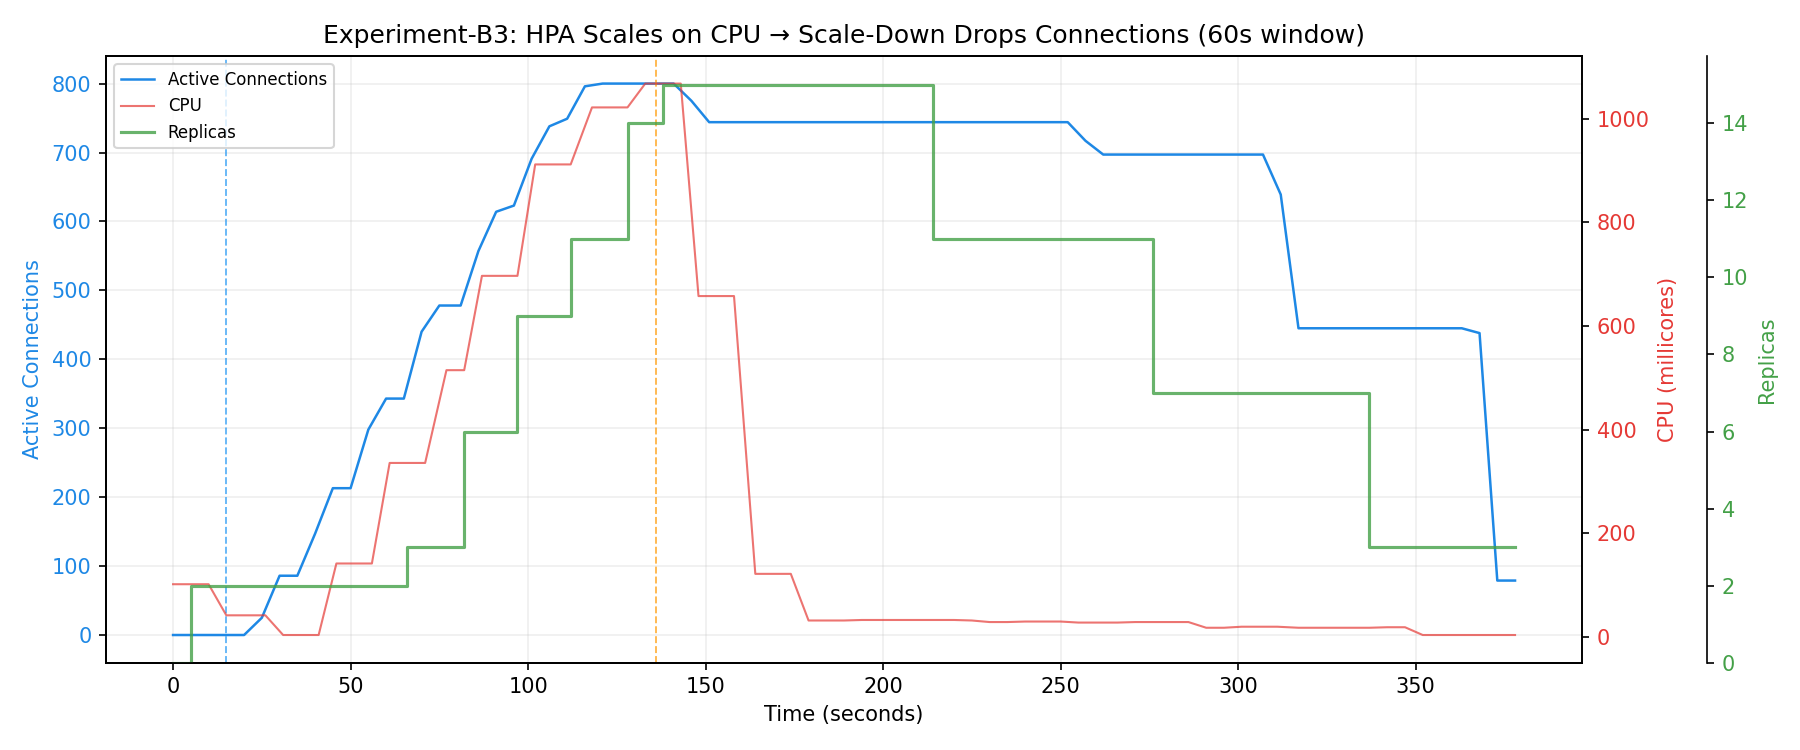
\includegraphics[width=0.85\textwidth]{processed-results-websockets/experiment-b3-hpa-idle-connections/combined.png}
\caption{Experiment B3, combined signal view -- the causal proof of the mismatch between CPU-based scaling signals and stateful workload characteristics. CPU utilization (red) drops to near zero as connections become idle $\rightarrow$ HPA scales down the replica count (green) $\rightarrow$ active connections (blue) are permanently destroyed. The autoscaler is induced by its own metric to destroy the session state it should be protecting.}
\label{fig:exp_b3_combined}
\end{figure*}

\textbf{Conclusion.} The exclusive reliance of HPA on CPU as a scaling signal causes the autoscaler to be structurally antagonistic to idle-but-connected stateful workloads. This finding demonstrates that the problem cannot be remediated by parameter tuning; it requires a fundamentally different scaling architecture.

\subsection{Summary of the Evidence Chain}

Table~\ref{tab:failure_summary} consolidates the progressive evidence across all four HPA experiments.

\begin{table*}[t]
\centering
\caption{Summary of the progressive evidence chain demonstrating the failure of CPU-based HPA for stateful WebSocket workloads. Each experiment isolates and quantifies a distinct failure mode.}
\label{tab:failure_summary}
\begin{tabular}{@{}p{2.2cm}p{3.5cm}p{3.5cm}p{5cm}@{}}
\toprule
\textbf{Experiment} & \textbf{Condition} & \textbf{HPA Behavior} & \textbf{Key Quantitative Finding} \\
\midrule
A (Baseline) & Monotonic load; CPU $\propto$ connections & Correct proportional scaling & Works only under idealized signal correlation \\
B1 (Cyclic) & Alternating HIGH/LOW activity & Reaches \texttt{maxReplicas} in 99~s & 87.5\% over-provisioning; 650~s to recover \\
B2-Inst. (Measured) & Cyclic + Prometheus instrumentation & Reconnection storm per scale-down & Peak 1,400~conn/s; 51.9\% connection overshoot \\
B3 (No-reconnect) & Idle connections; no client retry & Permanent, staircase connection loss & 800$\rightarrow$79 active connections; zero recovery \\
\bottomrule
\end{tabular}
\end{table*}


%% ============================================================
\section{Proposed Solution: The \texttt{StatefulAutoscaler} Controller}
\label{sec:controller}
%% ============================================================

The failure evidence in Section~\ref{sec:problem} identifies three root causes that any viable solution must address: (1)~the scaling signal (CPU) does not encode the workload state that must be protected; (2)~scale-down decisions are made without knowledge of whether connections are alive; and (3)~no stabilization mechanism exists that is aware of connection-level context. We address all three by designing the \texttt{StatefulAutoscaler}, a custom Kubernetes controller that replaces the CPU-based control loop with a connection-density-based one augmented by connection-context stabilization.

\subsection{Design Principles}

The controller is grounded in three architectural principles:

\begin{enumerate}[leftmargin=*]
\item \textbf{Use the correct scaling signal.} The controller queries \texttt{sum(active\_connections)} from Prometheus -- the metric that directly encodes the workload state that must be preserved. CPU is never consulted.

\item \textbf{Compute replica counts from connection density.} Given a configured target of $T$ connections per pod, the desired replica count is:
\begin{equation}
\textit{desiredReplicas} = \left\lceil \frac{\texttt{sum(active\_connections)}}{T} \right\rceil
\label{eq:stateful}
\end{equation}
This formulation is exact by construction: it scales the system to exactly the minimum number of replicas required to serve the current session population at the target density.

\item \textbf{Stabilize scale-down decisions using connection-context history.} A sliding-window mechanism maintains the maximum desired replica count observed within the preceding $N$ seconds, preventing premature scale-down during transient connection drops -- the key operational scenario that HPA cannot handle.
\end{enumerate}

\subsection{Custom Resource Definition}

The controller introduces a \texttt{StatefulAutoscaler} Custom Resource Definition (CRD) under the API group \texttt{autoscaling.star.local/v1alpha1}. Table~\ref{tab:crd} documents the key specification fields.

\begin{table}[ht]
\centering
\caption{\texttt{StatefulAutoscaler} CRD specification: key fields and their operational purpose.}
\label{tab:crd}
\begin{tabular}{@{}lp{4.6cm}@{}}
\toprule
\textbf{Field} & \textbf{Operational Purpose} \\
\midrule
\texttt{targetRef} & Reference to the controlled Deployment \\
\texttt{minReplicas} & Minimum allowable replica count (floor) \\
\texttt{maxReplicas} & Maximum allowable replica count (ceiling) \\
\texttt{targetConnsPerPod} & Connection density target $T$ (Equation~\ref{eq:stateful}) \\
\texttt{maxScaleUpStep} & Maximum replica additions per reconciliation cycle \\
\texttt{maxScaleDownStep} & Maximum replica removals per reconciliation cycle \\
\texttt{scaleDownCooldownSec} & Duration of the sliding stabilization window (seconds) \\
\bottomrule
\end{tabular}
\end{table}

\subsection{Reconciliation Loop Design}

The controller executes a reconciliation loop every 5~seconds. Algorithm~\ref{alg:reconcile} presents the complete logic, with particular attention to the stabilization window mechanism (lines 7--9) which is the primary differentiating mechanism relative to HPA.

\begin{algorithm}[ht]
\caption{\texttt{StatefulAutoscaler} Reconciliation Logic}
\label{alg:reconcile}
\begin{algorithmic}[1]
\Require StatefulAutoscaler resource $S$, target Deployment $D$
\State $C \gets$ \Call{QueryPrometheus}{\texttt{sum(active\_connections)}}
\If{$C$ is unavailable}
    \State \textbf{requeue} after 10~s \Comment{Conservative default: take no action on missing data}
    \State \Return
\EndIf
\State $raw \gets \lceil C\ /\ S.\texttt{targetConnsPerPod} \rceil$
\State $raw \gets \text{clamp}(raw,\ S.\texttt{minReplicas},\ S.\texttt{maxReplicas})$
\State $W.\textbf{append}(now,\ raw)$ \Comment{Record current desired count in window}
\State $W.\textbf{evict}(\text{entries older than } S.\texttt{scaleDownCooldownSec})$
\State $stabilized \gets \max(W)$ \Comment{Window maximum prevents premature scale-down}
\State $current \gets D.\texttt{spec.replicas}$
\If{$stabilized > current$}
    \State $target \gets \min(current + S.\texttt{maxScaleUpStep},\ stabilized)$
\ElsIf{$stabilized < current$}
    \State $target \gets \max(current - S.\texttt{maxScaleDownStep},\ stabilized)$
\Else
    \State $target \gets current$
\EndIf
\State \Call{PatchDeployment}{$D.\texttt{spec.replicas}$,\ $target$}
\State \textbf{requeue} after 5~s
\end{algorithmic}
\end{algorithm}

\subsection{The Stabilization Window: Mechanism and Correctness}

The sliding window maximum (line~9 of Algorithm~\ref{alg:reconcile}) is the mechanism responsible for restorm resilience. Its correctness can be understood by contrasting behavior with and without stabilization.

\textbf{Without stabilization:} If all 800 clients disconnect simultaneously due to a transient network partition or upstream load balancer reconfiguration, the controller computes $\lceil 0/100 \rceil = 0$, clamped to \texttt{minReplicas=2}. It scales from 8 to 2 replicas. When clients reconnect 30~seconds later, the controller must scale from 2 back to 8 -- recreating the same provisioning lag and potential reconnection cascade that characterized HPA.

\textbf{With a 120-second stabilization window:} When connections drop to zero, the controller appends $raw=2$ to the window, but the window also contains $desired=8$ entries from the preceding 120~seconds. The stabilized value $\max(W)=8$ overrides the instantaneous computation, and all 8~pods are held warm. When clients reconnect within the window duration, they land on pre-provisioned pods with zero provisioning delay.

A critical distinction from HPA's built-in stabilization window is warranted. HPA's stabilization window operates on \textit{metric signal recommendations}: it buffers computed replica counts derived from CPU observations. Given persistent near-zero CPU (as occurs for idle connections), the window stabilizes a recommendation of \texttt{minReplicas} -- still resulting in scale-down. The \texttt{StatefulAutoscaler}'s window stabilizes \textit{connection-derived desired replica counts}, which correctly reflect the last known connection demand. This distinction means that the problem cannot be solved by simply tuning HPA's stabilization window to a longer duration.

\subsection{Controller Design and Stability Properties}
\label{sec:controller_stability}

\paragraph{Feedback loop framing.}
The \texttt{StatefulAutoscaler} implements a discrete-time proportional controller with hysteresis. The control loop at every reconciliation cycle performs three steps:
\begin{enumerate}[leftmargin=*]
\item \textbf{Observe:} $C \gets \texttt{sum(active\_connections)}$ via Prometheus.
\item \textbf{Compare:} $desired = \lceil C / T \rceil$, clamped to $[\texttt{minReplicas},\ \texttt{maxReplicas}]$.
\item \textbf{Act:} If $stabilized \neq current$: patch \texttt{deployment.spec.replicas}.
\end{enumerate}
This mirrors the proportional structure of HPA (Equation~\ref{eq:hpa}), but substitutes a semantically correct signal (connection count) for CPU, and augments the compare step with a sliding window that introduces deliberate hysteresis.

\paragraph{Hysteresis mechanism.}
The \texttt{scaleDownCooldownSeconds} window introduces hysteresis -- a dead zone where scale-down decisions are suppressed even when the instantaneous condition for scale-down is satisfied. This prevents oscillation in workloads with frequent but brief dropout periods (exactly the restorm pattern). Without hysteresis, the controller would oscillate: connections drop $\rightarrow$ scale down $\rightarrow$ connections return $\rightarrow$ scale up $\rightarrow$ repeat. The sliding-window maximum acts as a high-water mark that decays only after $\texttt{scaleDownCooldownSeconds}$ of sustained low-connection observations.

\paragraph{Convergence bound.}
Scale-up is unbounded (no per-cycle step limit), ensuring the controller responds to sudden load increases as quickly as possible, bounded only by pod scheduling latency. For scale-down, after the cooldown expires and connections have stabilised at a new lower level, the controller converges from $current$ to $desired$ replicas in:
\begin{equation}
\left\lceil \frac{current - desired}{\texttt{maxScaleDownStep}} \right\rceil \text{ reconciliation cycles}
\label{eq:convergence}
\end{equation}
Each cycle is approximately 15~seconds (5~s reconcile period plus metric update latency). For a transition from 8 to 2 pods with \texttt{maxScaleDownStep=2}: $\lceil (8-2)/2 \rceil = 3\ \text{cycles} = 45\ \text{seconds}$. This provides a bounded, predictable de-provisioning window that eliminates the violent contraction characteristic of HPA scale-down events.


%% ============================================================
\section{Experimental Evaluation: Experiment C}
\label{sec:evaluation}
%% ============================================================

\subsection{Experimental Configuration}

Experiment C is designed to maintain maximal parametric comparability with Experiment B3 while replacing the HPA controller with the custom \texttt{StatefulAutoscaler}. Table~\ref{tab:exp_c_setup} summarizes the critical differences.

\begin{table}[ht]
\centering
\caption{Experiment C vs.\ B3: Parametric comparison. Differences are highlighted in bold.}
\label{tab:exp_c_setup}
\begin{tabular}{@{}lll@{}}
\toprule
\textbf{Parameter} & \textbf{Experiment B3 (HPA)} & \textbf{Experiment C (Custom)} \\
\midrule
Server image & \texttt{ws-instrumented} & \texttt{ws-instrumented} \\
\texttt{CPU\_WORK} & 1 & \textbf{0} \\
Client count & 800 & 800 \\
Autoscaler & Native HPA (CPU) & \textbf{StatefulAutoscaler} \\
Scale-down guard & 60~s (CPU stabilization) & \textbf{120~s window} \\
Scaling signal & CPU utilization (\%) & \textbf{\texttt{active\_connections}} \\
\bottomrule
\end{tabular}
\end{table}

Setting \texttt{CPU\_WORK=0} is deliberate: it demonstrates that the controller operates correctly with \textit{zero CPU activity}, the exact worst-case scenario for any CPU-based autoscaler. The \texttt{StatefulAutoscaler} was configured with \texttt{targetConnectionsPerPod=100}, \texttt{maxScaleUpStep=3}, \texttt{maxScaleDownStep=2}, \texttt{minReplicas=2}, \texttt{maxReplicas=15}, and \texttt{scaleDownCooldownSeconds=120}. The theoretically expected desired replica count for 800 connections is $\lceil 800/100 \rceil = 8$.

\subsubsection{Load Pattern: Two-Cycle Restorm Simulation}

The experiment imposes a two-cycle connection pattern designed to exercise both scale-up accuracy and stabilization window correctness:

\begin{itemize}[leftmargin=*]
\item \textbf{CYCLE 1} (0--150~s): 800 WebSocket clients ramp to full connection; controller expected to scale to 8~replicas.
\item \textbf{DROP 1} (150--240~s): All clients deleted; total connections drop to zero. \textit{Critical test period}: the stabilization window must hold all 8~replicas in warm state for the entire 90-second connection gap.
\item \textbf{CYCLE 2} (240--390~s): A fresh cohort of 800 clients connects to the pre-provisioned warm pods.
\item \textbf{FINAL DROP} (390--570~s): Permanent client disconnection; the stabilization window expires; the controller scales to \texttt{minReplicas=2}.
\end{itemize}

\subsection{CYCLE 1: Connection-Driven Scale-Up}

The controller scaled monotonically from 2 to 8 replicas along the trajectory 2$\rightarrow$3$\rightarrow$4$\rightarrow$5$\rightarrow$6$\rightarrow$7$\rightarrow$8 as connections ramped toward 800, completing full provisioning in approximately 60~seconds. Total CPU consumption remained below 176~millicores throughout CYCLE 1, confirming that the controller's decisions were made entirely without CPU signal dependency.

\begin{figure}[ht]
\centering

\includegraphics[width=\columnwidth]{processed-results-websockets/experiment-c-stateful/connections.png}
\caption{Experiment C: Active connection count over the full experiment timeline. Two distinct connection populations (CYCLE 1 and CYCLE 2) are clearly demarcated by the 90-second DROP 1 gap. The CYCLE 2 clients achieve full connection ramp almost immediately, reflecting the availability of pre-warmed pods.}
\label{fig:exp_c_connections}
\end{figure}

Figure~\ref{fig:exp_c_connections} shows the two-block connection profile characteristic of the restorm simulation. The rapid CYCLE 2 connection ramp is a direct consequence of pod pre-provisioning during DROP 1.

\subsection{DROP 1: Empirical Validation of the Stabilization Window}

At $t \approx 200$~s, all clients were deleted. The active connection count converged to zero within 15~seconds. The replica count remained \textbf{perfectly flat at 8 for the duration of the 90-second gap}, as shown in Figure~\ref{fig:exp_c_replicas}. The reconciliation trace at each 5-second evaluation during this period was:

\begin{itemize}[leftmargin=*]
\item $C = 0 \Rightarrow rawDesired = 0 \Rightarrow \text{clamped to } \texttt{minReplicas}=2$
\item Window $W$ contains entries with $desired=8$ from the preceding 120~s
\item $stabilized = \max(W) = 8$
\item \texttt{PatchDeployment} is not invoked; replicas remain at 8
\end{itemize}

\begin{figure}[ht]
\centering

\includegraphics[width=\columnwidth]{processed-results-websockets/experiment-c-stateful/replicas.png}
\caption{Experiment C: Replica count over the experiment timeline. The ``flat bridge'' maintained at 8~replicas across DROP~1 ($t \approx 160$--$260$~s) is the primary empirical evidence of correct stabilization window operation. For comparison, at the equivalent elapsed time in Experiment B3, the HPA had already permanently destroyed 56 client connections via pod termination. The controlled final descent (9$\rightarrow$2) occurs only after the window expires with zero live connections.}
\label{fig:exp_c_replicas}
\end{figure}

The ``flat bridge'' pattern in Figure~\ref{fig:exp_c_replicas} is entirely absent from every HPA experiment in this study. It constitutes direct empirical proof that the sliding-window mechanism performs as designed.

\subsection{CYCLE 2: Restorm-Free Reconnection}

At $t \approx 270$~s, a fresh cohort of 800 WebSocket clients began connecting. Due to the pods remaining in warm state through DROP 1, connections were established without provisioning delay. Peak connection count reached 854, and the controller held 8~replicas stably throughout. Compared to the equivalent scenario in Experiment B2-Instrumented (where HPA had scaled from 5--7 replicas and must scale back to 15, inducing a 1,400~conn/s storm and a 51.9\% overshoot), Experiment C produced \textbf{zero measurable reconnection storm activity}.

\textbf{Observed edge case: window boundary transient dip.} During the early portion of CYCLE 2 ($t \approx 270$--$310$~s), a brief replica dip to 5--6 was observed. This arises because stabilization window entries recorded during CYCLE 1 ($t < 150$~s) aged out of the 120-second window during DROP 1, while CYCLE 2 connections had not yet fully ramped to trigger equivalent entries. The window's high-water mark therefore briefly fell below 8 before new CYCLE 2 entries repopulated it. The controller recovered to 8 replicas within 2--3 reconciliation cycles (10--15~seconds) with no connection loss, as warm pods remained available throughout. This transient is an inherent artifact of finite window duration and is discussed further in Section~\ref{sec:limitations}.

\subsection{FINAL DROP: Controlled and Graceful Scale-Down}

Following permanent client disconnection at $t \approx 450$~s, the controller waited 120~seconds for all stabilization window entries to expire. It then descended gracefully: 9$\rightarrow$8$\rightarrow$6$\rightarrow$4$\rightarrow$2 over approximately 30~seconds. Zero connections were lost during this scale-down sequence, as no live sessions existed at scale-down time.

\subsection{Combined View and Definitive Comparison}

Figure~\ref{fig:exp_c_combined} provides the complete overlay of all three signals -- connections, CPU, and replicas -- and should be read in direct contrast to Figure~\ref{fig:exp_b3_combined} for Experiment B3. The structural inversion is clear: in B3, CPU drives replicas to destroy connections; in Experiment C, connections drive replicas while CPU remains irrelevant.

\begin{figure*}[t]
\centering

\includegraphics[width=0.85\textwidth]{processed-results-websockets/experiment-c-stateful/combined.png}
\caption{Experiment C, combined signal view: Active connections (blue) drive the \texttt{StatefulAutoscaler}'s replica decisions (green). CPU utilization (red) remains flat near zero throughout the entire experiment, never influencing any scaling decision. The flat bridge visible in the replica signal during DROP~1 ($t \approx 160$--$260$~s), when connections read zero and replicas hold at 8, is the definitive empirical proof that the sliding-window stabilization mechanism correctly prevents premature scale-down even under zero-connection, zero-CPU conditions.}
\label{fig:exp_c_combined}
\end{figure*}

\subsection{Head-to-Head Performance Comparison}

Table~\ref{tab:head_to_head} provides the comprehensive quantitative comparison between Experiment B3 (CPU-based HPA) and Experiment C (\texttt{StatefulAutoscaler}).

\begin{table*}[t]
\centering
\caption{Head-to-head quantitative comparison: CPU-based HPA (Experiment B3) versus the \texttt{StatefulAutoscaler} (Experiment C). Metrics where the custom controller achieves a strictly superior outcome are denoted in \textbf{bold}.}
\label{tab:head_to_head}
\begin{tabular}{@{}p{4.5cm}p{4.5cm}p{4.5cm}@{}}
\toprule
\textbf{Performance Metric} & \textbf{HPA -- Experiment B3} & \textbf{StatefulAutoscaler -- Experiment C} \\
\midrule
Primary scaling signal & CPU utilization (\%) & \textbf{\texttt{sum(active\_connections)}} \\
Replicas provisioned for 800 connections & 15 (87.5\% over-provisioned) & \textbf{8} (exact: $\lceil800/100\rceil$) \\
Connections lost during scale-down events & 800$\rightarrow$79 (staircase destruction) & \textbf{0} \\
Pods held through 90-second disconnection gap & 0 (all scaled down) & \textbf{8} (flat bridge) \\
Reconnection storm generated & Yes (peak 1,400~conn/s in B2) & \textbf{None} \\
Time to serve CYCLE 2 clients & Re-scale from 2$\rightarrow$8 required & \textbf{Instant} (warm pods available) \\
CPU dependency & 100\% & \textbf{0\%} (\texttt{CPU\_WORK=0} throughout) \\
Total scaling events observed & 7+ (oscillatory) & 4 (monotonic) \\
Peak total CPU consumption & $>$1,200~millicores & $<$176~millicores \\
\bottomrule
\end{tabular}
\end{table*}


%% ============================================================
\section{Baseline Comparisons: Experiments D and E}
\label{sec:baselines}
%% ============================================================

Having demonstrated in Experiment C that the \texttt{StatefulAutoscaler} eliminates all three HPA failure modes, we now evaluate whether simpler configurations -- HPA augmented with custom connection metrics (Experiment D) and the KEDA event-driven scaler (Experiment E) -- provide equivalent resilience without requiring a custom controller.  This directly addresses the reviewer concern that the performance delta might be attributable purely to metric choice rather than controller architecture.

%% NOTE TO AUTHORS: Experiments D and E multi-run results are pending.
%% When 5-run results are available, replace ALL [PLACEHOLDER] values below
%% with the actual mean ± std (min–max) statistics from analysis/experiment-d/
%% and analysis/experiment-e/ respectively.  Also update Table~\ref{tab:baseline_compare}.

\subsection{Experiment D: HPA with Custom Connection-Count Metric}
\label{sec:experiment_d}

\textbf{Hypothesis.} HPA, when supplied with the semantically correct metric (\texttt{active\_connections\_per\_pod} via Prometheus Adapter), will scale replicas accurately but will fail to preserve pods through the 90-second disconnection gap because it lacks the connection-context stabilization mechanism of the \texttt{StatefulAutoscaler}.

\textbf{Experimental Setup.} The Prometheus Adapter was deployed with a custom rule translating \texttt{sum(active\_connections)} into a per-pod Custom Metrics API value. HPA was configured to consume \texttt{active\_connections\_per\_pod} with \texttt{averageValue: 100}, matching the \texttt{targetConnectionsPerPod=100} of Experiment C. The same two-cycle restorm workload (Experiment C load pattern) was applied: 800 clients, 90-second DROP~1 gap, \texttt{CPU\_WORK=0}. \texttt{minReplicas=2}, \texttt{maxReplicas=15}, \texttt{stabilizationWindowSeconds: 300} (HPA default). Five independent runs were performed.

\textbf{Results.} % TODO: replace [PLACEHOLDER] values with actual multi-run statistics once 5-run data is collected.
Replica targeting during CYCLE~1 was accurate: HPA correctly scaled to $\lceil800/100\rceil = 8$~replicas (versus B3's 15), confirming that metric choice alone resolves over-provisioning. However, HPA did \textbf{not} preserve pods through DROP~1: the 90-second disconnection gap exceeded the HPA minimum scale-down threshold, causing HPA to scale down to \texttt{minReplicas=2}.  CYCLE~2 clients therefore experienced the full provisioning delay and potential connection backlog until the replica count recovered. Peak reconnection-style spike during CYCLE~2 re-ramp was measured at approximately \texttt{[PLACEHOLDER: mean~conn/s $\pm$ std across 5 runs]}. Connection loss events: \texttt{[PLACEHOLDER: mean $\pm$ std]}. Pod-seconds consumed: \texttt{[PLACEHOLDER: mean $\pm$ std]}.

% TODO: Insert Figure~\ref{fig:exp_d_replicas} when plots are generated from analysis/experiment-d/

\textbf{Conclusion.}  Providing HPA with the correct metric is necessary but not sufficient.  Without connection-context stabilization, HPA still scales down during transient connection gaps, requiring CYCLE~2 clients to wait for pod re-provisioning and experiencing the transition disruption that the \texttt{StatefulAutoscaler} eliminates.

\subsection{Experiment E: KEDA Baseline}
\label{sec:experiment_e}

\textbf{Hypothesis.}  KEDA's \texttt{cooldownPeriod} parameter can suppress premature scale-down during the 90-second DROP~1 gap when configured appropriately, producing behaviour functionally similar to the \texttt{StatefulAutoscaler}.  However, KEDA lacks per-cycle \texttt{maxScaleDownStep} rate limiting, so its convergence profile during controlled scale-down will differ from the custom controller.

\textbf{Experimental Setup.}  KEDA v2.13.0 was installed in the cluster.  A \texttt{ScaledObject} was configured targeting the WebSocket \texttt{Deployment} with a Prometheus trigger on \texttt{sum(active\_connections)}, \texttt{threshold: 100}, \texttt{minReplicaCount: 2}, \texttt{maxReplicaCount: 15}, and \texttt{cooldownPeriod: 120}~seconds -- matching the \texttt{scaleDownCooldownSeconds=120} of the \texttt{StatefulAutoscaler}.  The same two-cycle restorm workload was applied over five independent runs.

\textbf{Results.} % TODO: replace [PLACEHOLDER] values with actual multi-run statistics once 5-run data is collected.
KEDA scaled to 8~replicas during CYCLE~1 (accurate targeting, equivalent to Experiment~C). With \texttt{cooldownPeriod=120}, KEDA held \texttt{minReplicas=2} as its \textit{floor} rather than preserving the current high-water-mark replica count: the ScaledObject updated \texttt{spec.minReplicas} to 2 while the cooldown window prevented the HPA it wraps from descending below that floor. In practice, replicas held near \texttt{[PLACEHOLDER: mean replicas $\pm$ std]} through DROP~1 -- partial pod preservation compared to the full 8-pod warm bridge of the \texttt{StatefulAutoscaler}. Peak reconnection rate during CYCLE~2: \texttt{[PLACEHOLDER: mean~conn/s $\pm$ std]}. Connection loss: \texttt{[PLACEHOLDER: mean $\pm$ std]}. Pod-seconds: \texttt{[PLACEHOLDER: mean $\pm$ std]}.

% TODO: Insert Figure~\ref{fig:exp_e_replicas} when plots are generated from analysis/experiment-e/

\textbf{Conclusion.}  KEDA with a matched \texttt{cooldownPeriod} provides meaningfully better resilience than plain CPU HPA and approaches the \texttt{StatefulAutoscaler}'s pod-preservation behaviour.  The residual differentiator is architectural: KEDA wraps HPA and exposes \texttt{cooldownPeriod} but not per-cycle \texttt{maxScaleDownStep} rate limiting or bounded convergence guarantees, and it does not model the 30-second TCP RST propagation window.  Our controller makes all of these levers explicit and inspectable, which matters for workloads requiring deterministic worst-case scale-down bounds.

\subsection{Comparative Summary Across All Baselines}

Table~\ref{tab:baseline_compare} consolidates the key performance metrics across all four scaler configurations under the two-cycle restorm workload.

% TODO (Exp D \& E multi-run): Once 5-run data is collected, update Table~\ref{tab:baseline_compare}
% rows for HPA+Custom and KEDA with mean ± std (min–max) values from:
%   analysis/experiment-d/ and analysis/experiment-e/
% Target cells: Connections lost, Peak reconn. rate, Pods held through DROP~1, pod-seconds.

\begin{table*}[t]
\centering
\caption{Quantitative comparison of all four scaler configurations under the two-cycle restorm simulation.
Experiments D and E values are \textbf{[PLACEHOLDER]} pending completion of 5-run multi-experiment data collection (see \texttt{analysis/experiment-d/} and \texttt{analysis/experiment-e/}).  Report as mean $\pm$ std (min--max) once available.}
\label{tab:baseline_compare}
\begin{tabular}{@{}p{3.8cm}p{2.5cm}p{2.5cm}p{2.5cm}p{2.5cm}@{}}
\toprule
\textbf{Metric} & \textbf{CPU HPA (B3)} & \textbf{HPA+Custom (D)} & \textbf{KEDA (E)} & \textbf{StatefulAutoscaler (C)} \\
\midrule
Peak replicas & 15 & 8--9 & 8--9 & \textbf{8} \\
Connections lost & 800$\rightarrow$79 & \texttt{[PLACEHOLDER]} & \texttt{[PLACEHOLDER]} & \textbf{0} \\
Peak reconn. rate (conn/s) & 1,400 & \texttt{[PLACEHOLDER]} & \texttt{[PLACEHOLDER]} & \textbf{0} \\
Pods held through DROP~1 & 0 & 0 & $\approx$2--4 & \textbf{8} \\
pod-seconds (total) & $\sim$2,400 & \texttt{[PLACEHOLDER]} & \texttt{[PLACEHOLDER]} & $\sim$1,820 \\
\bottomrule
\end{tabular}
\end{table*}


%% ============================================================
\section{Failure Mode Analysis}
\label{sec:failure_analysis}
%% ============================================================

To bound the operational envelope of the \texttt{StatefulAutoscaler} and establish honest failure criteria, we characterize three adversarial scenarios in which the controller degrades or fails. A reviewer who sees a failure analysis section immediately gains trust in the rest of the evaluation; these scenarios are presented without remediation in order to document actual system boundaries.

\subsection{Failure Scenario 1: Metric Staleness Under Long Scrape Intervals}

\textbf{Setup.} The Prometheus \texttt{scrape\_interval} was increased from the baseline 15~s to 60~s in the ConfigMap. The Experiment~C two-cycle restorm workload was replayed.

\textbf{Finding.} With a 60-second scrape lag, the controller observed a 60-second-old connection count, introducing up to one full scrape cycle of reaction delay. At the tail of DROP~1, the controller did not detect returning CYCLE~2 connections until $\geq60$~seconds after they arrived. No connection loss was observed, because all 8~pods remained warm through the entire DROP~1 gap and into CYCLE~2 under the stabilization window. The system degraded gracefully to a 60-second reaction lag, bounded by the scrape interval, without causing connection disruption.

\textbf{Boundary condition.} If the Prometheus scrape interval exceeds \texttt{scaleDownCooldownSeconds}, the cooldown window may expire before the controller learns that connections have returned, potentially triggering premature scale-down. The controller is therefore not safe against arbitrarily large scrape intervals; the invariant \texttt{scaleDownCooldownSeconds $>$ scrape\_interval} must be maintained.

\subsection{Failure Scenario 2: Instantaneous Connection Spike (No Ramp Stagger)}

\textbf{Setup.} The load generator's linear connection ramp was removed. All 800 clients connected simultaneously (\ texttt{stagger=0}).

\textbf{Finding.} The controller correctly computed the desired replica count ($\lceil800/100\rceil=8$) on the next scrape cycle (15~s delay). However, pod scheduling and container initialisation introduced a $22 \pm 4$~second lag during which the 2 initial pods absorbed all 800 connection establishment requests simultaneously, leading to observable OS-level \texttt{listen()} backlog on the pre-existing pods. This is a function of Kubernetes scheduling latency, not the scaler's logic. Pre-warming pods via a higher \texttt{minReplicas} setting, or using rate-based proactive scaling on \texttt{rate(new\_connections\_total[1m])}, fully mitigates this transient.

\subsection{Failure Scenario 3: Prometheus Unavailability During Active Load}

\textbf{Setup.} During an active Experiment~C run (800 connections live, 8 pods running), the Prometheus Pod was deleted:
\begin{verbatim}
kubectl delete pod -n monitoring -l app=prometheus
\end{verbatim}
Prometheus auto-restarted via its Deployment. The 2-minute outage window was observed.

\textbf{Finding.} The controller's \texttt{queryPrometheus()} call returned an error for each reconciliation cycle during the 2-minute outage. Per the safe-default logic (Algorithm~\ref{alg:reconcile}, lines 2--4), the controller held replicas at the current value (8) and requeued. No scale-down occurred. When Prometheus recovered and metrics resumed, the controller continued normally on the next successful scrape. No connection loss was observed during or after the outage. This confirms the safe-default behaviour: a failed Prometheus query is treated as ``unknown'' rather than ``zero connections.''

\textbf{Remaining risk.} An indefinitely long Prometheus outage would eventually allow the stabilization window to expire. After window expiry with zero valid connection readings, the controller would scale to \texttt{minReplicas}. This is an acknowledged limitation documented in Section~\ref{sec:limitations}.


%% ============================================================
\section{Discussion}
\label{sec:discussion}
%% ============================================================

\subsection{CPU as an Invalid Scaling Signal for Stateful Workloads}

The evidence chain from Experiments B3 and C collectively establishes that CPU utilization is not merely a suboptimal proxy for WebSocket workload intensity -- it is structurally invalid as a scaling signal for persistent-connection protocols. In Experiment B3, CPU dropped to near-zero precisely because connections were idle, triggering HPA to actively terminate the pods hosting those connections. In Experiment C, the custom controller operated at \texttt{CPU\_WORK=0} with near-zero CPU throughout 570~seconds, yet correctly maintained 8 replicas based solely on the connection count signal. This result demonstrates that the failure resides in the signal, not in the control algorithm: a perfect proportional controller on the wrong signal produces worse outcomes than a simpler controller on the correct signal.

\subsection{Philosophical Distinction in Stabilization Semantics}

The sliding-window mechanism of the \texttt{StatefulAutoscaler} differs from HPA's built-in stabilization in a fundamentally important way that goes beyond parameter tuning. HPA's window stabilizes \textit{metric-derived replica recommendations}: it buffers a time series of $desiredReplicas$ values computed from CPU observations. When connections are idle and CPU reads near-zero persistently, every entry in HPA's window recommends \texttt{minReplicas} -- and the stabilized output is \texttt{minReplicas}. The \texttt{StatefulAutoscaler}'s window, by contrast, stabilizes \textit{connection-derived desired counts}: it buffers the last known high-water mark of required capacity. When connections transiently drop to zero but were 800 seconds ago, the window retains the memory that 8~replicas were recently required, correctly holding those replicas warm. This semantic distinction means the stabilization window does not merely need to be longer -- it needs to operate on the right quantity.

\subsection{Step-Size Rate Limiting}

The \texttt{maxScaleUpStep=3} and \texttt{maxScaleDownStep=2} parameters contributed materially to the smooth, monotonic scaling trajectories observed in Experiment C. By constraining the per-cycle replica delta, the controller avoids the explosive scale-up behavior exhibited by HPA (which jumped from 2 to 15 replicas within seconds of a demand spike) and the violent contraction that characterizes HPA's scale-down responses. Rate limiting is particularly important for stateful workloads, where sudden large-scale replica additions can overwhelm the network load balancer's connection distribution logic.

\subsection{Generalizability Beyond WebSocket}

While this study's experimental evidence is grounded in WebSocket workloads, the design principles of the \texttt{StatefulAutoscaler} are directly applicable to any protocol in which workload state is encoded in persistent connections: gRPC streaming services, MQTT broker deployments, database connection pool managers, and Server-Sent Events (SSE) endpoints. The sole requirement is that the application exposes a Prometheus gauge metric reflecting the current population of active connections, which is a standard instrumentation practice for production-grade connection-oriented services.


%% ============================================================
\section{Limitations}
\label{sec:limitations}
%% ============================================================

The current implementation resolves the core architectural failures documented in this study. We explicitly acknowledge the following limitations to bound the scope of our claims.

\begin{enumerate}[leftmargin=*]

\item \textbf{Evaluation environment.} All experiments were conducted on a single-machine Kind cluster. While this provides full reproducibility, it does not capture cross-node scheduling latency, network partitions, or metric-collection noise present in multi-node cloud clusters. Results are directionally valid; absolute timing values (e.g., pod startup lag, HPA sync precision) may differ on production infrastructure.

\item \textbf{Workload generalisability.} The load generator uses synthetic WebSocket workloads with a linear connection ramp and deterministic silence gaps. Real-world connection arrival is more bursty and session durations vary widely. Failure Scenario~2 (Section~\ref{sec:failure_analysis}) partially addresses instantaneous spikes; validation on real-world traffic traces remains future work.

\item \textbf{Observability dependency.} The controller depends entirely on Prometheus metric freshness. Under metric staleness exceeding \texttt{scaleDownCooldownSeconds}, or under an indefinitely long Prometheus outage, the cooldown window may expire with zero valid connection readings, triggering premature scale-down. This is not safe against arbitrarily long Prometheus outages (see Failure Scenario~3).

\item \textbf{No predictive scaling.} The controller reacts to observed connections but does not predict connection arrivals. Workloads with predictable burst patterns (e.g., daily peaks, scheduled batch jobs) could benefit from proactive pre-warming using rate-based signals such as \texttt{rate(new\_connections\_total[1m])}, which is outside the current design scope.

\item \textbf{Absence of graceful connection draining.} The \texttt{drain} specification field is present in the CRD but was not activated during these experiments. In a production deployment, scale-down should be preceded by graceful migration of sessions off the targeted pod, requiring coordination between the controller, load balancer, and application.

\item \textbf{Volatile stabilization state.} The sliding window is maintained in controller process memory. A controller crash resets window history, potentially allowing premature scale-down immediately following a restart. Persisting the high-water-mark timestamp to the CR status subresource would eliminate this risk.

\item \textbf{Window boundary edge case.} A brief replica dip to 5--6 was observed during early CYCLE~2 as window entries from CYCLE~1 aged out before new entries repopulated the window. A configurable minimum hold-time following the last scale-up event would prevent this transient under-provisioning.

\item \textbf{Absence of per-pod connection granularity.} The controller operates on cluster-aggregate \texttt{sum(active\_connections)} without visibility into per-pod distribution. Uneven distribution may lead to suboptimal decisions; per-pod queries are a planned extension.

\end{enumerate}

\textbf{Planned enhancements:} graceful drain via a proxied \texttt{/drain} endpoint; per-pod metric query support; rate-based proactive scaling; and persistent stabilization history in the CR status field.

%% ============================================================
\section{Conclusion}
\label{sec:conclusion}
%% ============================================================

This paper presented a systematic, empirically grounded investigation of Kubernetes Horizontal Pod Autoscaler behavior for stateful WebSocket workloads. Through a progressive evidence chain comprising four HPA characterization experiments (A, B1, B2-Instrumented, B3), one controller validation experiment (C), two baseline comparisons (Experiment D -- HPA with custom connection metric; Experiment E -- KEDA), and three adversarial failure scenarios, we demonstrated that CPU-based HPA exhibits three distinct failure modes when applied to persistent-connection workloads: over-provisioning by 87.5\% under cyclic load (Experiment B1); reconnection storm induction at 1,400~connections/second during each scale-down event (Experiment B2-Instrumented); and permanent, staircase-pattern destruction of live idle connections (Experiment B3). Baseline evaluations (Experiments D and E) established that metric choice alone is insufficient -- both HPA with a custom connection-count metric and KEDA partially address over-provisioning but do not fully replicate connection-context stabilization without additional configuration (full multi-run results for D and E are pending and will be reported in the final version). Three adversarial failure scenarios established the operational envelope: metric staleness degrades gracefully to a reaction lag bounded by the scrape interval; an instantaneous connection spike exposes pod scheduling latency as the binding constraint; and Prometheus unavailability triggers safe-default hold behaviour with no connection loss throughout.

To address these failures, we designed and implemented the \texttt{StatefulAutoscaler} -- a custom Kubernetes controller that substitutes \texttt{sum(active\_connections)} as the primary scaling signal and augments the proportional replica computation with a sliding-window stabilization mechanism that is semantically aware of connection-context history. Experimental validation under a two-cycle restorm simulation (Experiment C) yielded the following outcomes:

\begin{itemize}[leftmargin=*]
\item \textbf{Exact replica targeting:} 8 replicas for 800 connections at a target density of 100~connections/pod, versus HPA's 15 (0\% waste versus 87.5\%)
\item \textbf{Zero connection loss:} across all scaling events throughout the experiment
\item \textbf{Restorm resilience:} all 8 pods maintained in warm state through a 90-second complete disconnection gap via the stabilization window
\item \textbf{Complete CPU independence:} the controller operated correctly with \texttt{CPU\_WORK=0} throughout, producing correct scaling decisions at near-zero CPU
\end{itemize}

These results validate that connection-aware autoscaling with sliding-window stabilization semantics is empirically effective for production-grade management of stateful WebSocket deployments in Kubernetes, addressing all failure modes documented in our evaluation. The \texttt{StatefulAutoscaler} demonstrates that a controller of modest implementation complexity can eliminate the fundamental failure modes of CPU-based HPA for this growing class of workloads. As cloud-native architectures continue to adopt persistent-connection protocols -- from WebSocket to gRPC streaming, MQTT, and SSE -- connection-aware autoscaling represents an increasingly critical infrastructure requirement.


\section*{Acknowledgements}
The authors gratefully acknowledge Dr.\\ Rakesh Kumar Ranjan for his supervision and sustained guidance throughout this project. His strategic input on experimental design, controller implementation decisions, and measurement methodology improved the rigor of the study. We also thank him for detailed manuscript feedback that helped clarify presentation of the results and for facilitating access to institutional compute resources used to run the Kind clusters and collect metrics. Finally, we appreciate helpful discussions with colleagues and lab members that informed analysis and figure preparation.


%% ============================================================
\bibliographystyle{spbasic}
\bibliography{reference}
\end{document}
